% Draft manuscript for MNRAS (revision 1, after internal referee review, 2026-11-22).
% Compile with mnras.cls (e.g. Overleaf "MNRAS template"):
%   pdflatex main && bibtex main && pdflatex main && pdflatex main
% Every number comes from results/ : h1_results.json, h1_robustness.csv, h1_hierarchical.txt,
% h1_extra.json, method_check.md, outburst_table.csv, timescales_maxi.csv (see paper/notes.md).

\documentclass[fleqn,usenatbib]{mnras}
\usepackage[T1]{fontenc}
\usepackage{newtxtext,newtxmath}
\usepackage{graphicx}
\usepackage{amsmath}
\usepackage{booktabs}
\usepackage[hidelinks]{hyperref}

\newcommand{\taud}{\tau_{\rm d}}
\newcommand{\taur}{\tau_{\rm r}}
\newcommand{\porb}{P_{\rm orb}}
\newcommand{\dex}{\,dex}

\title[BH transient decay times vs orbital period]{Disc size is not the main factor in the decay: outburst timescales of black hole X-ray transients in the MAXI era and a statistical test against orbital period}

\author[B. {[Surname]}]{Berkh [Surname]$^{1}$\thanks{E-mail: [author e-mail]}
\\
$^{1}$Independent researcher, [City, Country]}

\date{Accepted XXX. Received YYY; in original form ZZZ}
\pubyear{2026}

\begin{document}
\label{firstpage}
\pagerange{\pageref{firstpage}--\pageref{lastpage}}
\maketitle

\begin{abstract}
In the irradiated disc instability model, a black hole transient decays on the viscous time of its hot disc, so systems with longer orbital periods, and larger discs, should decay more slowly. We test this. We measure two-point e-folding rise and decay times (the Yan \& Yu 2015 definition) for black hole and candidate outbursts observed by MAXI and Swift/BAT, giving a catalogue of 55 outburst windows from 2016--2026, with 24 unconfused bright main outbursts from 13 sources. We validate the method against two published samples and with injection--recovery in real MAXI data, fix the analysis plan, and combine our values with RXTE-era measurements for systems with independently measured periods: 26 outbursts of 13 systems with $\porb=0.10$--$2.62$\,d. The slope of $\log\taud$ against $\log\porb$ is $B=0.17$ (95 per cent interval $-0.17$ to $0.52$), so the predicted increase is not detected. Standard disc scalings predict $B\approx2/3$--$5/6$; slopes of $2/3$ or more have posterior probability 0.006 and are excluded in every leave-one-system-out fit. A shallower slope near $1/3$ remains allowed. Outbursts of the same system scatter by 0.27\dex, as much as systems scatter about the fit (0.24\dex), so the period is at most a minor factor. We also find that two groups applying the same method to the same RXTE data differ by up to a factor of 4.6, and that a published 2019 outburst of GS~1354$-$64 is MAXI~J1348$-$630.
\end{abstract}

\begin{keywords}
accretion, accretion discs -- black hole physics -- X-rays: binaries -- stars: black holes -- methods: statistical
\end{keywords}

%=====================================================================
\section{Introduction}
\label{sec:intro}

Most dynamically confirmed black holes in the Galaxy were discovered as X-ray transients in low-mass X-ray binaries \citep{CorralSantana2016}. These systems spend years to decades in quiescence and then brighten by several orders of magnitude for weeks to months \citep{Tetarenko2016}. The outbursts are explained by the disc instability model. The accretion disc stores mass while it is cool and neutral; when hydrogen ionizes somewhere in the disc, the viscosity rises sharply and the disc drains on to the black hole \citep{Lasota2001,Hameury2020}. In X-ray binaries the central X-rays also irradiate the outer disc, keeping it ionized and prolonging the outburst \citep{KingRitter1998,Dubus2001}.

\citet{KingRitter1998} showed that irradiation sets the shape of the decay. While the X-rays keep the whole disc hot, the disc mass, and with it the luminosity, falls exponentially on the viscous time of the hot region, $\tau\simeq R_{\rm h}^2/3\nu$. Here $R_{\rm h}$ is the radius of the irradiated, ionized region and $\nu$ the kinematic viscosity. Once the luminosity falls below the value needed to ionize the disc to its edge, the hot region shrinks and the decay becomes linear \citep{KingRitter1998,Shahbaz1998}. The outer disc radius is a fixed fraction of the Roche lobe, which grows with orbital period, so this picture predicts slower exponential decays in longer-period systems. The decay time could therefore probe disc size and the viscosity of the hot disc \citep{Tetarenko2018a,Tetarenko2018b}.

Two uniform studies have tested this prediction, and they disagree. \citet{YanYu2015} measured two-point e-folding times for 110 outbursts of 36 transients (black holes and neutron stars) observed by the RXTE All-Sky Monitor \citep[ASM;][]{Levine1996} in 1996--2011. They found that the rise time correlates with orbital period but the decay time does not. \citet{Saraswati2025} applied the same definition to outbursts and smaller `mini-outbursts' of nine dynamically confirmed black holes observed with ASM and MAXI up to 2024. They reported that the decay time increases with orbital period, but gave no statistical test.

Since 2016, the Monitor of All-sky X-ray Image \citep[MAXI;][]{Matsuoka2009,Mihara2011} and the Swift Burst Alert Telescope transient monitor \citep[BAT;][]{Krimm2013} have observed many new black hole outbursts with daily cadence. Several of these systems now have orbital periods from optical spectroscopy, for example MAXI~J1820+070 \citep{Torres2019} and Swift~J1727.8$-$1613 \citep{MataSanchez2025}. A recent MAXI and BAT study of 42 low-mass X-ray binaries \citep{Maheshwari2026} measured hardness and outburst durations, but not decay timescales or their relation to orbital period. We have found no published study that tests the decay-time--period relation formally, with measurement errors, intrinsic scatter, model comparison and a power estimate, on a sample that includes the post-2016 outbursts.

This paper makes that test. Our aims are:
\begin{enumerate}
\item to build a uniform catalogue of rise and decay timescales for black hole and candidate outbursts observed by MAXI in 2016--2026, with the \citet{YanYu2015} definition so that it can be merged with the earlier samples;
\item to validate the measurement against both earlier samples and against simulated outbursts in real MAXI data, before running the test;
\item to test, with a plan fixed in advance, whether the decay time increases with orbital period (hypothesis H1).
\end{enumerate}
Section~\ref{sec:theory} derives the slope that the irradiated disc model predicts. Section~\ref{sec:data} describes the data and sample, and Section~\ref{sec:method} the measurements, validation and statistics. Section~\ref{sec:results} presents the results, Section~\ref{sec:discussion} discusses them, and Section~\ref{sec:conclusions} summarizes.

%=====================================================================
\section{The expected slope}
\label{sec:theory}

We write the decay time as a power law in orbital period, $\taud\propto\porb^{B}$, and estimate $B$. With the $\alpha$ prescription \citep{ShakuraSunyaev1973}, $\nu=\alpha c_{\rm s}H=\alpha c_{\rm s}^2/\Omega_{\rm K}$, where $c_{\rm s}$ is the sound speed, $H$ the scale height and $\Omega_{\rm K}=(GM/R^3)^{1/2}$ the Keplerian angular frequency \citep{FrankKingRaine2002}. The e-folding time of \citet{KingRitter1998} becomes
\begin{equation}
\tau\simeq\frac{R_{\rm h}^2}{3\nu}=\frac{(GM)^{1/2}\,R_{\rm h}^{1/2}}{3\,\alpha\,c_{\rm s}^2}\propto\frac{M^{1/2}R_{\rm h}^{1/2}}{\alpha\,T(R_{\rm h})},
\label{eq:tau}
\end{equation}
where $T(R_{\rm h})$ is the midplane temperature at $R_{\rm h}$ and $M$ the black hole mass. During the exponential phase the whole disc is ionized, so $R_{\rm h}$ is the outer disc radius. Tides limit this radius to a fixed fraction of the Roche lobe of the accretor \citep[][who use 80 per cent]{Shahbaz1998}. The Roche-lobe radius is a fraction of the binary separation $a$ that depends only on the mass ratio \citep{Eggleton1983}, and Kepler's third law gives $a\propto(M_{\rm tot}\porb^2)^{1/3}$. At fixed masses, therefore, $R_{\rm h}\propto\porb^{2/3}$.

The slope then depends on how $\alpha T(R_{\rm h})$ changes from a small disc to a large one. We consider three cases.
\begin{itemize}
\item \textit{Irradiation-dominated disc.} If the outer disc temperature is set by irradiation, $T^4\propto L/R^2$ at a given luminosity $L$ \citep{Dubus1999}, so $T(R_{\rm h})\propto R_{\rm h}^{-1/2}$. Then $\tau\propto R_{\rm h}$ and $B=2/3$.
\item \textit{Viscously heated disc.} For a gas-pressure-dominated disc with Kramers opacity, $\nu\propto R^{3/4}$ at a given accretion rate \citep{ShakuraSunyaev1973,FrankKingRaine2002}. Then $\tau\propto R_{\rm h}^{5/4}$ and $B=5/6$.
\item \textit{Edge pinned at the ionization temperature.} If $\alpha T$ at the disc edge is the same in every system, for example because the edge sits close to the hydrogen ionization temperature, then $\tau\propto R_{\rm h}^{1/2}$ and $B=1/3$. This applies only near the end of the exponential phase, when the luminosity approaches the critical value and the edge is barely ionized.
\end{itemize}
The standard expectation for the exponential phase is therefore $B\approx2/3$--$5/6$, with $B\approx1/3$ as a shallow limiting case. Differences in luminosity, accretion rate and $\alpha$ between systems add scatter around these slopes. Differences in black hole mass also add scatter: in the edge-pinned case, equation~(\ref{eq:tau}) gives $\taud\propto M^{2/3}$ at fixed $\porb$, so a factor of two in mass changes $\taud$ by 0.2\dex; the other cases have a similar, weak mass dependence that also involves the luminosity or accretion rate.

Three effects can weaken the relation in real data. First, if the peak luminosity is too low to ionize the whole disc, $R_{\rm h}$ is set by the luminosity rather than by the orbit \citep{KingRitter1998,Shahbaz1998}. Second, disc winds remove mass and can shorten the decay independently of disc size \citep{Tetarenko2018a,Dubus2019}. Third, the model describes the accretion rate, while we measure the flux in a fixed X-ray band, which also changes with the spectral state.

%=====================================================================
\section{Data and sample}
\label{sec:data}

\subsection{Light curves}
\label{sec:lc}

We use the MAXI Gas Slit Camera (GSC) standard one-day light curves, which give count rates in the 2--4, 4--10 and 10--20\,keV bands for each catalogued source. Our primary band is 2--10\,keV, the sum of the 2--4 and 4--10\,keV rates, with errors added in quadrature. We convert rates to Crab units with the MAXI team's Crab rates (2.2 and 1.25\,ph\,cm$^{-2}$\,s$^{-1}$ in the two bands, so 1\,Crab $=3.45$\,ph\,cm$^{-2}$\,s$^{-1}$ in 2--10\,keV). This band differs from the 2--12\,keV band of ASM and of \citet{Saraswati2025}. Section~\ref{sec:val_results} measures the effect of this and other differences directly.

From the BAT transient monitor we use the daily 15--50\,keV light curves (1\,Crab $=0.220$\,count\,cm$^{-2}$\,s$^{-1}$). We keep only points with data flag 0 and remove two intervals with known problems (MJD 58571--58573 and 58736--58747). We use BAT to check the identity of sources that may be confused in MAXI, and to measure hard X-ray decay times as a secondary quantity.

\subsection{Outburst windows}
\label{sec:windows}

We find outbursts automatically in each MAXI light curve. A seven-point (seven-day) running median must exceed 0.05\,Crab to start a candidate, and candidates closer than 30\,d are merged. Each window is extended in both directions until the smoothed flux falls below the larger of 10 per cent of the peak and 0.01\,Crab, and is then padded by 15\,d. Where padded windows overlap, they are split at the midpoint. A window is also split when the flux falls below 25 per cent of the peak and then rises again above twice that minimum and above 0.05\,Crab; the later part is labelled a re-flare. Near the Galactic Centre the MAXI flux does not always return to zero between outbursts. We therefore subtract from each window a local baseline, the median flux within 60\,d on either side outside all outburst windows.

A short override file, kept with the code, records every manual decision with its reason. These cover the restriction of Swift~J1727.8$-$1613 to its 2023--24 outburst (earlier windows are noise, and BAT confirms only this outburst), the removal of two short spikes, the removal of Swift~J1753.5$-$0127 (its MAXI light curve contains only the end of its 2005--2017 outburst), and the flags for source confusion described in Section~\ref{sec:confusion}. The study window runs from 2016 January 1 (MJD 57388) to 2026 November. MAXI windows with earlier peaks (from 2009 August) are also measured; they are used in the validation and, under the plan's rule for choosing measurements (Section~\ref{sec:stats}), in the test.

\subsection{Sources and orbital periods}
\label{sec:sample}

We started from the black holes and candidates in BlackCAT \citep{CorralSantana2016} that were active after 2016. Our source table has 27 entries, each system parameter with its reference, and is part of the data release. Of the 24 sources with a MAXI standard light curve, 19 show at least one outburst window.

For the test of H1 we use only systems whose orbital period was measured independently of the X-ray decay: by optical spectroscopy, optical photometry, H$\alpha$ modulation or X-ray dips. We exclude MAXI~J0637$-$430, whose 2.2\,h period was inferred from its own outburst decay \citep{Soria2022}, because using it would make the test circular. Neutron stars are excluded. Swift~J1357.2$-$0933 has a period \citep{CorralSantana2013} but never exceeded our brightness limit in MAXI. Table~\ref{tab:sample} lists the 13 systems in the test, with periods from 0.100\,d (MAXI~J1659$-$152) to 2.62\,d (GRO~J1655$-$40). Ten have radial-velocity orbits. GRS~1716$-$249 has a photometric period, and its mass estimate uses an H$\alpha$ line-width relation rather than a full radial-velocity curve \citep{Casares2023}. The two candidates, MAXI~J1659$-$152 and MAXI~J1803$-$298, have periods from X-ray dips.

\begin{table*}
\centering
\caption{Systems in the decay-time--period test, numbered by period as in Fig.~\ref{fig:taup}. $n$ is the number of bright outbursts, and $\langle\taud\rangle=10^{\langle\log\taud\rangle}$ over those outbursts. Origin: TW = this work (MAXI), YY = \citet{YanYu2015}, S = \citet{Saraswati2025}. For the five systems marked $^{a}$, the period is the value tabulated in the compilation named, where the original measurement is cited. $^{b}$Photometric period; mass from an H$\alpha$ line-width relation, not a full radial-velocity orbit.}
\label{tab:sample}
\begin{tabular}{rlcllcccl}
\toprule
\# & System & $\porb$ (d) & Method & Status & $n$ & $\langle\taud\rangle$ (d) & Origin & Period reference \\
\midrule
1 & MAXI J1659$-$152   & 0.1004 & X-ray dips & candidate & 1 & 14.2 & TW & \citet{YanYu2015}$^{a}$; \citet{Kuulkers2013} \\
2 & Swift J1753.5$-$0127 & 0.1358 & spectroscopy & dynamical & 1 & 28.5 & YY & \citet{YanesRizo2025} \\
3 & XTE J1859+226      & 0.274 & spectroscopy & dynamical & 1 & 17.2 & YY & \citet{YanYu2015}$^{a}$ \\
4 & GRS 1716$-$249     & 0.278 & photometry & dynamical$^{b}$ & 1 & 75.0 & TW & \citet{Casares2023} \\
5 & MAXI J1803$-$298   & 0.2925 & X-ray dips & candidate & 1 & 15.6 & TW & \citet{Jana2022} \\
6 & XTE J1650$-$500    & 0.318 & spectroscopy & dynamical & 1 & 29.1 & YY & \citet{YanYu2015}$^{a}$ \\
7 & Swift J1727.8$-$1613 & 0.4502 & spectroscopy & dynamical & 1 & 35.3 & TW & \citet{MataSanchez2025} \\
8 & MAXI J1820+070     & 0.6855 & spectroscopy & dynamical & 1 & 35.8 & TW & \citet{Torres2019} \\
9 & 4U 1543$-$47       & 1.1164 & spectroscopy & dynamical & 2 & 22.9 & TW, YY & \citet{Orosz1998,Orosz2003} \\
10 & XTE J1550$-$564   & 1.542 & spectroscopy & dynamical & 3 & 15.4 & S, YY & \citet{Saraswati2025}$^{a}$ \\
11 & GX 339$-$4        & 1.7588 & spectroscopy & dynamical & 10 & 49.2 & TW, S, YY & \citet{Heida2017} \\
12 & GS 1354$-$64      & 2.5445 & spectroscopy & dynamical & 1 & 26.3 & TW & \citet{Casares2009} \\
13 & GRO J1655$-$40    & 2.622 & spectroscopy & dynamical & 2 & 81.1 & S, YY & \citet{Saraswati2025}$^{a}$ \\
\bottomrule
\end{tabular}
\end{table*}

\subsection{Literature timescales}
\label{sec:literature}

We transcribed the black hole entries of \citet[][their tables 1 and 8; 42 outbursts]{YanYu2015} and table~2 of \citet[][33 outbursts and mini-outbursts]{Saraswati2025}. Nine outbursts appear in both papers, which we identify by source and by peak dates within 15\,d of each other. For these we take the mean of the two values of $\log\taud$. Section~\ref{sec:val_results} shows that the two papers can disagree strongly about the same outburst.

%=====================================================================
\section{Methods}
\label{sec:method}

\subsection{Two-point e-folding timescales}
\label{sec:tau}

We follow the definition of \citet{YanYu2015}, also used by \citet{Saraswati2025}. Between two points on the decay with fluxes $F_1>F_2$ at times $t_1<t_2$, the e-folding time is
\begin{equation}
\tau=\frac{t_2-t_1}{\ln(F_1/F_2)},
\label{eq:twopoint}
\end{equation}
and the rise time is defined in the same way on the rise. We use the daily points closest to 90, 50 and 10 per cent of the daily peak flux, which give $\tau_{10-90}$, $\tau_{10-50}$ and $\tau_{50-90}$. Our primary quantity is $\taud\equiv\tau_{\rm d,10-90}$.

The selection rule matters for reproducibility, so we state it in full. Before selection we remove isolated spikes: points more than twice, or less than half, the flux of both neighbours, and points whose error is more than twice that of both neighbours. On the decay, the 90 per cent point is the point closest to 0.9 of the peak, searched from the peak until two consecutive points fall below 0.8. The 50 per cent point is searched from the first point below 0.66 until two consecutive points fall below 0.33. The 10 per cent point is searched from the first point below 0.20 until two consecutive points fall below 0.01, or until the window ends. The rise is treated in mirror image. In equation~(\ref{eq:twopoint}) we use the measured flux ratio of the selected points, not the nominal ratio, so that a point that misses its level does not bias $\tau$.

For a pure exponential the three timescales are equal. For a linear decay the flux takes equal times to fall from 90 to 50 and from 50 to 10 per cent, so $\tau_{50-90}/\tau_{10-50}=\ln5/\ln1.8\simeq2.7$. We call this ratio the shape ratio. As a secondary estimate, we also find the 90, 50 and 10 per cent crossing times by linear interpolation on a three-point running median. An outburst counts as bright if its daily peak exceeds 0.1\,Crab, the limit of \citet{YanYu2015}, by at least three times the peak error. This is a flux cut only: an event that \citet{Saraswati2025} call a mini-outburst enters if it passes it. Fig.~\ref{fig:lc} shows four examples.

\begin{figure*}
\centering
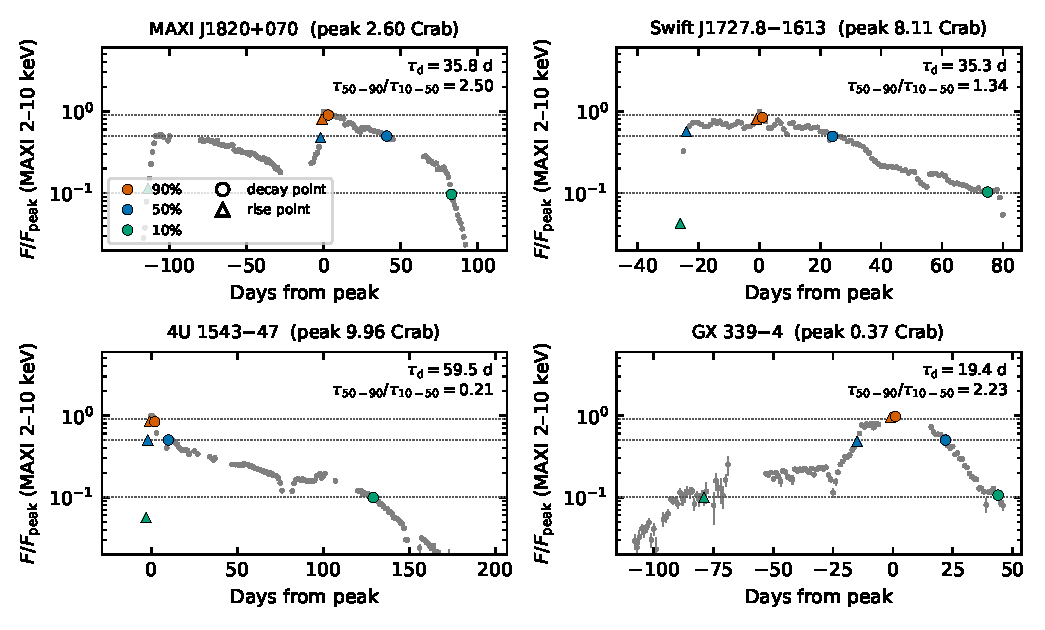
\includegraphics[width=\textwidth]{figures/fig1_lightcurves.pdf}
\caption{Four MAXI 2--10\,keV light curves from the catalogue, normalized to the daily peak and baseline-subtracted. Coloured symbols mark the points selected at 90, 50 and 10 per cent of the peak on the rise (triangles) and the decay (circles); dotted lines show the three levels. Each panel gives $\taud\equiv\tau_{\rm d,10-90}$ and the shape ratio, which is 1 for an exponential and about 2.7 for a linear decay. Swift~J1727.8$-$1613 decays nearly exponentially; MAXI~J1820+070 and GX~339$-$4 (2024) steepen; 4U~1543$-$47 (2021) slows down. For MAXI~J1820+070 the 2--10\,keV peak is the later soft-state peak, so its rise points span the whole preceding hard state.}
\label{fig:lc}
\end{figure*}

\subsection{Uncertainties}
\label{sec:errors}

We estimate errors by Monte Carlo: each light curve is resampled 300 times within its flux errors and all timescales are remeasured, and we quote the 16th and 84th percentiles. The two-point estimator is discontinuous, because a small change in flux can move the selection to a different day. The resampled distribution is therefore not always centred on the value measured from the data; for 6 of the 24 outbursts in Table~\ref{tab:catalogue} the measured value lies outside its own 16--84 per cent range. We keep the measured value as the estimate and use half the 16--84 per cent width, in dex, as its uncertainty, with a floor of 0.02\dex.

For the literature values we convert the published errors to dex, apply the same floor, and add in quadrature a method term $\sigma_{\rm method}=0.19$\dex. The published errors describe photon noise only, and do not cover differences in how the 90, 50 and 10 per cent points are chosen. The value 0.19\dex\ was fixed in the plan as the largest robust scatter in the original validation comparisons (0.195\dex, this work against \citealt{YanYu2015}; Section~\ref{sec:val_results}). Because plain standard deviations are larger (0.18--0.25\dex), the plan also tests $\sigma_{\rm method}=0.3$\dex.

\subsection{Validation}
\label{sec:validation}

Before running the test of H1, we compared our measurements with both literature samples and tested the estimator on simulated outbursts. We required agreement within the errors, or an explained offset, before going on.
\begin{enumerate}
\item \textit{This work against \citet{YanYu2015}}: five outbursts in 2009--2010 observed by both ASM and MAXI.
\item \textit{This work against \citet{Saraswati2025}}: their MAXI-era outbursts whose peak lies inside one of our windows, excluding the confused event of Section~\ref{sec:confusion} (eight outbursts).
\item \textit{\citet{YanYu2015} against \citet{Saraswati2025}}: nine outbursts that both groups measured from the same ASM data. This comparison measures how reproducible the method is between groups when the data are identical.
\item \textit{Injection--recovery}: we injected synthetic outbursts with exponential rise and decay into quiescent stretches of real MAXI 2--10\,keV data from four sources (MAXI~J1820+070, GRS~1716$-$249, H1743$-$322 and EXO~1846$-$031), keeping the real cadence, gaps and noise. Peaks were 0.1, 0.3, 1 and 3\,Crab and true decay times 5--80\,d, with 48 realizations per combination, and each was measured with the same code as the real outbursts.
\end{enumerate}

\subsection{Statistical test}
\label{sec:stats}

\textit{Plan.} We wrote the analysis plan after the validation and recorded its SHA-256 fingerprint (2026 November 21, 21:54 UTC) before the first test. According to file timestamps, two implementation clarifications were appended to the plan, and the table of literature periods was finalized, in the following two minutes, before the first result was produced (21:57 UTC). The recorded fingerprint matches the plan text without the appended section. The plan was not deposited in an external registry, so these times cannot be verified independently. All files are part of the data release.

\textit{Sample.} The plan fixes the primary sample as all bright outbursts of systems with an independent period, excluding re-flares and outbursts affected by source confusion. Failed outbursts that never reach the soft state are included. For each outburst our MAXI value is used if we measured it, whatever its date. Otherwise we use the mean of $\log\taud$ from the two literature samples, or the single available value.

\textit{Model.} Each system contributes one point, the mean of $\log\taud$ over its outbursts, so that a system with many outbursts (GX~339$-$4 has ten) does not dominate. Its measurement error is $\sigma_k^2=\sum_j\sigma_{jk}^2/n_k^2$ for system $k$ with $n_k$ outbursts. The model is
\begin{equation}
\log\taud=A+B\log(\porb/1\,{\rm d})+\epsilon,\qquad\epsilon\sim\mathcal{N}(0,\,\sigma_{\rm int}^2+\sigma_k^2),
\label{eq:model}
\end{equation}
where the intrinsic scatter $\sigma_{\rm int}$ is a free parameter \citep{Kelly2007}. We sample the posterior with \textsc{emcee} \citep{ForemanMackey2013}, with flat priors on $A\in[-1,4]$, $B\in[-3,3]$ and $\log\sigma_{\rm int}\in[-3,0.5]$. H1 is supported if the 95 per cent credible interval of $B$ lies above zero. Because H1 is one-sided, this is equivalent to requiring $P(B>0)>0.975$.

\textit{Model comparison.} We compare three models on the same data: M0, a constant ($B=0$); M1, the power law of equation~(\ref{eq:model}); and M2, a power law that saturates above a break, $\log\taud=A+B\min(x,x_{\rm b})$ with $x=\log(\porb/1\,{\rm d})$ and $x_{\rm b}$ free in $[-0.7,0.7]$. M2 represents a levelling-off of $\taud$ at long periods. The plan ranks the models by the Akaike and Bayesian information criteria \citep[AIC, BIC;][]{Akaike1974,Schwarz1978}, computed from the maximum likelihood, and by a leave-one-system-out (LOSO) log predictive density, in which each system is predicted from the maximum-likelihood fit to the others. As a test that ignores the error bars, we compute Kendall's rank correlation $\tau_{\rm K}$ between $\log\taud$ and $\log\porb$, with a $p$-value from 10\,000 random permutations of the periods (2000 for the robustness checks).

\textit{Power.} Before looking at the result, we estimated the power of the test. We simulated 200 data sets with the real periods and errors, a true slope $B$, and $\sigma_{\rm int}$ equal to the scatter of the literature-only sample about a constant (0.23\dex), and counted how often the 95 per cent interval of $B$ excluded zero. The plan specified $B=0.5$; we also ran $B=0.3$.

\textit{Robustness checks in the plan.} These are reported but not used to decide H1:
(i) including re-flares;
(ii) including faint outbursts, meaning all mini-outbursts and peaks below 0.1\,Crab;
(iii) dynamically confirmed black holes only;
(iv) our measurements only, and literature only;
(v) MAXI timescales without baseline subtraction;
(vi) timescales from smoothed crossings;
(vii) $\sigma_{\rm method}=0$ and 0.3\dex;
(viii) a hierarchical model on individual outbursts. This model has a random effect per system, $\log\tau_{jk}=A+B\,x_k+u_k+e_{jk}$, with $u_k\sim\mathcal{N}(0,\sigma_{\rm sys}^2)$ and $e_{jk}\sim\mathcal{N}(0,\sigma_{\rm out}^2+\sigma_{jk}^2)$. Here $\sigma_{\rm sys}$ is the real scatter between systems beyond the period dependence, and $\sigma_{\rm out}$ the real scatter between outbursts of one system. We integrate the $u_k$ out analytically and sample $A$, $B$, $\log\sigma_{\rm sys}$ and $\log\sigma_{\rm out}$ with flat priors (log-uniform for the scatters, lower bound $10^{-3}$\dex).
The rise time (H2) is tested in the same way, as an exploratory analysis.

\textit{Implementation clarifications.} Two details were added to the plan before the first result, without changing any rule. First, a literature outburst counts as measured by us if its peak date lies inside one of our outburst windows. This prevents double counting of multi-peaked outbursts, whose peaks in different bands can be more than 20\,d apart. Second, for MAXI-era literature outbursts that our detection did not find, the 0.1\,Crab limit is applied to our own 2--10\,keV data within 15\,d of the published peak.

\subsection{Checks added after the plan}
\label{sec:extra}

After an internal review of the first results, we added checks that are not part of the plan and that do not change the decision rule for H1:
(a) a posterior-predictive version of the LOSO score, in which each left-out system is predicted by averaging over the posterior of the fit to the other systems \citep[cf.][]{Vehtari2017}, and the small-sample AIC (AICc);
(b) the influence of each system on $B$, by refitting without it;
(c) the posterior probability of the theoretical slopes of Section~\ref{sec:theory};
(d) further variants: periods from radial-velocity orbits only; without the one Saraswati mini-outburst that passes our flux cut (XTE~J1550$-$564 in 2001, 0.11\,Crab); ASM values shifted by the measured offset of $+0.16$\dex\ (Section~\ref{sec:val_results}); the error of each discrepant duplicate raised to half the difference between the two published values; a per-system variance that includes an outburst-to-outburst term, $\sigma_k^2+\sigma_{\rm out}^2/n_k$ with $\sigma_{\rm out}=0.27$\dex\ from the hierarchical model; and the early-decay timescale $\tau_{\rm d,50-90}$, which samples the phase most likely to be exponential;
(e) the hierarchical model with half-normal priors (scale 0.5\dex) on $\sigma_{\rm sys}$ and $\sigma_{\rm out}$.
We also corrected one flag. The re-flare window of GS~1354$-$64 at MJD 58560 is the tail of the confused event of Section~\ref{sec:confusion} but had not been flagged. Flagging it changes only robustness check (i).

%=====================================================================
\section{Results}
\label{sec:results}

\subsection{The 2016--2026 catalogue}
\label{sec:catalogue}

We find 55 outburst windows from 17 sources in 2016--2026. Sixteen are flagged for source confusion (Section~\ref{sec:confusion}); thirteen of these are windows of MAXI~J1631$-$479, whose MAXI light curve repeats that of 4U~1630$-$47. Of the 39 unflagged windows, 24 are bright main outbursts from 13 sources (Table~\ref{tab:catalogue}); the others are re-flares or peaked below 0.1\,Crab. This set of 13 sources overlaps only partly with the 13 systems of the H1 test, because many catalogue sources have no measured period. The decay times of the 24 bright outbursts range from 15 to 86\,d, with a median of 31\,d. BAT decay times are shorter than MAXI decay times for most outbursts (median ratio 0.61 for the 18 outbursts with BAT values), as expected, because the hard X-ray flux falls quickly when a source enters the soft state. The full table, including flagged and faint windows, rise times, all three decay timescales and the dates and fluxes of the selected points, is part of the data release.

\begin{table*}
\centering
\caption{Bright ($>0.1$\,Crab in 2--10\,keV) main outbursts in 2016--2026 that are not affected by source confusion, in order of peak date. $F_{\rm pk}$ is the daily peak. $\taud$ is $\tau_{\rm d,10-90}$, with the 16--84 per cent Monte Carlo range in brackets; the range is not always centred on the measured value (Section~\ref{sec:errors}). SR is the shape ratio $\tau_{\rm d,50-90}/\tau_{\rm d,10-50}$, and $\tau_{\rm d}^{\rm BAT}$ the 15--50\,keV decay time. All times are in days. Rise times below about 2\,d are not resolved by daily sampling.}
\label{tab:catalogue}
\begin{tabular}{lcccccc}
\toprule
Source & Peak MJD & $F_{\rm pk}$ (Crab) & $\taur$ & $\taud$ & SR & $\tau_{\rm d}^{\rm BAT}$ \\
\midrule
4U 1630$-$47        & 57669.5 & 0.28 & 15.1  & 37.1 [35.1, 41.9] & 13.0 & 23.3 \\
GRS 1716$-$249      & 57821.5 & 0.26 & --    & 75.0 [67.3, 74.3] & 4.42 & 95.1 \\
MAXI J1535$-$571    & 58016.5 & 2.11 & 5.9   & 35.6 [35.7, 50.0] & 0.84 & -- \\
MAXI J1727$-$203    & 58277.5 & 0.18 & --    & 19.1 [16.5, 21.8] & 0.23 & 16.7 \\
MAXI J1820+070      & 58306.5 & 2.60 & 57.7  & 35.8 [34.7, 36.0] & 2.50 & 43.3 \\
4U 1630$-$47        & 58334.5 & 0.30 & 28.4  & 43.4 [39.3, 44.8] & 1.65 & 10.5 \\
MAXI J1348$-$630    & 58523.5 & 3.11 & 6.0   & 27.8 [27.8, 28.5] & 2.66 & -- \\
4U 1630$-$47        & 58687.5 & 0.16 & 7.3   & 19.9 [18.3, 20.6] & 3.06 & -- \\
EXO 1846$-$031      & 58705.5 & 0.44 & 5.5   & 65.9 [48.2, 65.4] & 2.01 & 17.0 \\
GX 339$-$4          & 58845.5 & 0.64 & 16.6  & 33.5 [31.5, 34.7] & 0.47 & 5.7 \\
4U 1630$-$47        & 58965.5 & 0.34 & 17.6  & 21.2 [19.4, 21.1] & 1.85 & 11.5 \\
GX 339$-$4          & 59332.5 & 0.61 & 36.2  & 50.5 [49.2, 61.7] & 0.40 & 4.4 \\
MAXI J1803$-$298    & 59349.5 & 0.52 & 5.6   & 15.6 [14.5, 30.9] & 0.46 & 6.3 \\
4U 1543$-$47        & 59379.5 & 9.96 & 0.7   & 59.5 [58.8, 60.0] & 0.21 & 0.9 \\
4U 1630$-$47        & 59498.5 & 0.39 & 9.3   & 15.3 [14.5, 17.9] & 3.29 & 21.1 \\
4U 1630$-$47        & 60008.5 & 0.67 & 115.3 & 85.9 [83.5, 92.4] & 0.11 & 9.5 \\
H1743$-$322         & 60016.5 & 0.26 & 2.3   & 18.5 [18.2, 20.1] & 0.32 & -- \\
Swift J1727.8$-$1613 & 60206.5 & 8.11 & 8.5  & 35.3 [34.2, 35.4] & 1.34 & 23.5 \\
GX 339$-$4          & 60351.5 & 0.37 & 34.6  & 19.4 [17.1, 19.6] & 2.23 & 14.6 \\
GX 339$-$4          & 60560.5 & 0.22 & 31.4  & 21.8 [22.7, 25.5] & 1.54 & 17.4 \\
4U 1630$-$47        & 60787.5 & 0.26 & 4.7   & 18.5 [15.2, 18.5] & 0.36 & 11.0 \\
GS 1354$-$64        & 61069.5 & 0.51 & 9.7   & 26.3 [26.1, 28.9] & 2.20 & 21.4 \\
H1743$-$322         & 61279.5 & 1.00 & 5.6   & 33.4 [22.2, 35.8] & 0.30 & -- \\
4U 1630$-$47        & 61292.5 & 0.56 & 2.7   & 23.1 [18.8, 23.3] & 2.60 & -- \\
\bottomrule
\end{tabular}
\end{table*}

\subsection{Validation}
\label{sec:val_results}

Fig.~\ref{fig:validation} and Table~\ref{tab:validation} summarize the validation. We give both a robust scatter, from the median absolute deviation (MAD), and the plain standard deviation (SD), because the comparisons contain a few large outliers.

Our MAXI values agree well with those of \citet{Saraswati2025} for most outbursts: the median offset is $-0.04$\dex\ and the robust scatter 0.05\dex\ ($N=8$). The SD is larger, 0.24\dex, because of two events. The faint 2022 mini-outburst of 4U~1543$-$47 peaked at only 0.06\,Crab in our band (4.6 against 20.4\,d), and the hard-state 2015 outburst of GS~1354$-$64 differs by 0.17\dex. Against \citet{YanYu2015}, our values have a median offset of $+0.16$\dex\ and a scatter of 0.18--0.20\dex\ ($N=5$). We traced the differences to two causes. For the faint 2010 outbursts of H1743$-$322 and MAXI~J1659$-$152, ASM noise at the 10 per cent level moves the selected point, and a re-flare of 4U~1630$-$47 was handled differently.

The comparison between the two published samples is the most informative. For nine outbursts measured from the same ASM data, the median offset is only $-0.05$\dex\ and the robust scatter 0.10\dex, but the SD is 0.25\dex\ because of large outliers. For the 1998 outburst of XTE~J1550$-$564, \citet{YanYu2015} give $\taud=19$\,d and \citet{Saraswati2025} give 89\,d, a factor of 4.6. For the 1996 outburst of GRO~J1655$-$40 the values are 172 and 97\,d. Both outbursts have several peaks, and the difference comes from which part of the light curve was taken as the decay. We return to this in Section~\ref{sec:repro}.

Injection--recovery shows that the estimator is unbiased in the MAXI data (Fig.~\ref{fig:validation}b). For decay times of 5--80\,d the median of $\log(\tau_{\rm meas}/\tau_{\rm true})$ lies within 0.035\dex\ of zero at all peak fluxes. The robust scatter is 0.07--0.10\dex\ at 0.1\,Crab and at most 0.04\dex\ at 0.3\,Crab and above, and at least 96 per cent of injections were recovered in every case. Photon noise and sampling are therefore small compared with the differences between outbursts found below. The simulations use single exponential outbursts only, so they do not test the choices that matter for multi-peaked outbursts.

\begin{figure*}
\centering
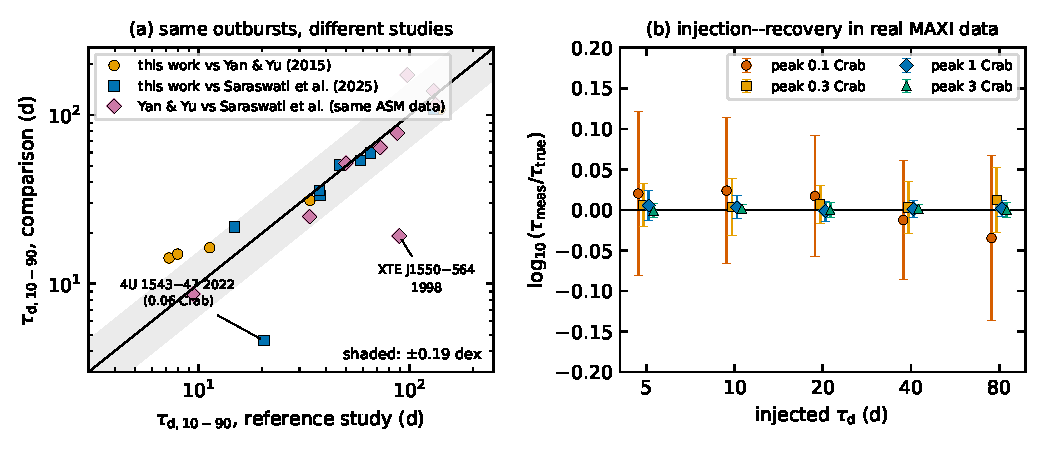
\includegraphics[width=\textwidth]{figures/fig2_validation.pdf}
\caption{Method validation. (a) $\taud$ for the same outbursts measured by different studies. For each series, the $x$-axis holds the second study named in the legend and the $y$-axis the first. The line shows equality and the shaded band $\pm0.19$\dex, the method uncertainty that we add to literature values. (b) Injection--recovery of exponential outbursts in real quiescent MAXI data: median and robust scatter of the log ratio of measured to true decay time for four peak fluxes (offset slightly in $x$ for clarity).}
\label{fig:validation}
\end{figure*}

\begin{table}
\centering
\caption{Agreement of $\taud$ between studies for the same outbursts: median $\log$ ratio (first study over second), robust scatter (1.4826 times the MAD) and standard deviation, all in dex.}
\label{tab:validation}
\begin{tabular}{lcccc}
\toprule
Comparison & $N$ & Median & MAD & SD \\
\midrule
This work / Yan \& Yu & 5 & $+0.16$ & 0.20 & 0.18 \\
This work / Saraswati et al. & 8 & $-0.04$ & 0.05 & 0.24 \\
Yan \& Yu / Saraswati et al. & 9 & $-0.05$ & 0.10 & 0.25 \\
\bottomrule
\end{tabular}
\end{table}

\subsection{Decay time against orbital period (H1)}
\label{sec:h1}

The primary sample contains 26 bright outbursts of 13 systems: 13 outbursts measured by us with MAXI and 13 from the literature. The power analysis, done before the test, gave a probability of 0.84 to detect a true slope of $B=0.5$ and 0.39 to detect $B=0.3$, each with a Monte Carlo uncertainty of about 0.03.

Fig.~\ref{fig:taup}a shows the result. The posterior slope is $B=0.17$, with a 95 per cent interval of $-0.17$ to $0.52$. The normalization is $A=1.52$ (1.34--1.69), which corresponds to $\taud=33$\,d at $\porb=1$\,d, and the intrinsic scatter is $\sigma_{\rm int}=0.24$\dex\ (0.15--0.41). The interval of $B$ includes zero, so H1 is not supported. The posterior probability of a positive slope is 0.85. Kendall's rank correlation is $\tau_{\rm K}=0.31$, with a permutation $p=0.16$.

The model comparison does not separate the models strongly (Table~\ref{tab:h1}). AIC is 4.26 for M0, 4.91 for M1 and 5.60 for M2; AICc, which corrects for the small sample, is 5.46, 7.58 and 10.60; BIC gives the same order. Differences of 1--2 in these criteria are weak evidence. The planned LOSO score, with maximum-likelihood predictions, is $-2.36$ for M0, against $-5.67$ for M1 and $-6.97$ for M2. This large gap comes almost entirely from GRS~1716$-$249. When it is left out, the maximum-likelihood fit of M1 to the other systems has a small intrinsic scatter, which makes its prediction for GRS~1716$-$249 very confident and very wrong. The posterior-predictive LOSO score, which averages over the uncertainty in the fit, is less sensitive to this: $-2.17$ for M0, $-3.18$ for M1 and $-2.79$ for M2. All the criteria rank the constant model first, but only by small margins, and GRS~1716$-$249 also accounts for most of the gap in the posterior-predictive score. The maximum-likelihood fit of M2 puts the break at the lower edge of its range ($\porb=0.2$\,d), with all the slope below it, so it follows the two shortest-period systems rather than describing a levelling-off at long periods.

\begin{figure*}
\centering
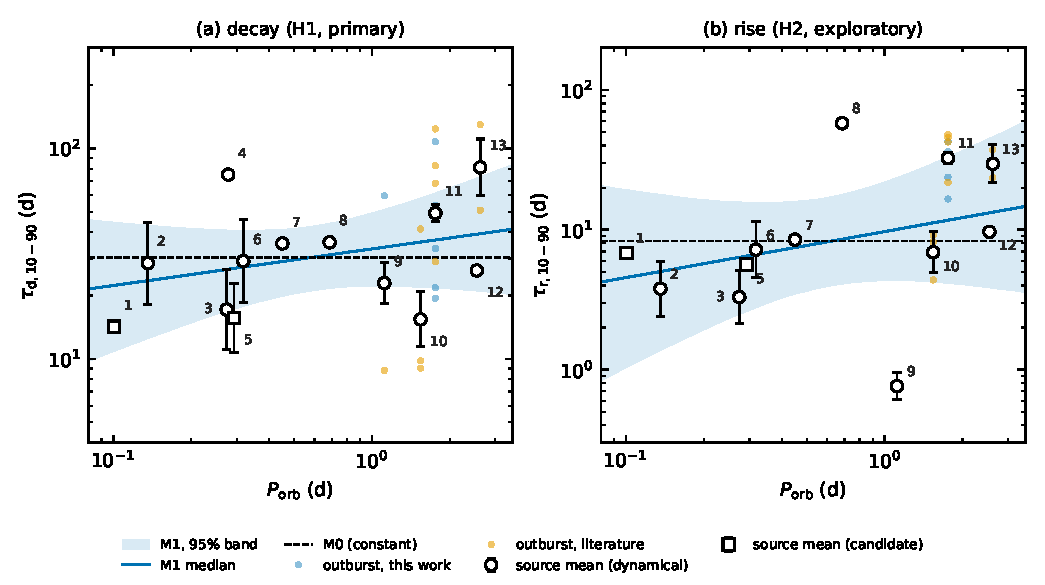
\includegraphics[width=\textwidth]{figures/fig3_tau_porb.pdf}
\caption{Outburst timescales against orbital period. (a) Decay time $\taud$ (H1). Small dots are individual outbursts (blue: this work; orange: literature). Large open symbols are system means (circles: dynamically confirmed; squares: candidates), numbered as in Table~\ref{tab:sample}. Their error bars show measurement errors only; the fitted intrinsic scatter, 0.24\dex, is not included. The blue line and band show the median and 95 per cent range of the power-law model M1, and the dashed line the constant model M0. (b) The same for the rise time $\taur$ (H2, exploratory; 12 systems).}
\label{fig:taup}
\end{figure*}

\begin{table*}
\centering
\caption{Test of H1. Upper part: model comparison for the primary sample (lower AIC, AICc and BIC, and higher LOSO, are better). Lower part: posterior median and 95 per cent interval of $B$, and Kendall's $\tau_{\rm K}$ with its permutation $p$-value. $N_{\rm s}$ and $N_{\rm o}$ are the numbers of systems and outbursts. The primary row uses 10\,000 permutations and the other rows 2000; Kendall's $\tau_{\rm K}$ ignores errors, so it is the same for all rows with the same data.}
\label{tab:h1}
\begin{tabular}{lccccc}
\toprule
Model & AIC & AICc & BIC & LOSO (plan, ML plug-in) & LOSO (posterior predictive) \\
\midrule
M0 constant & 4.26 & 5.46 & 5.39 & $-2.36$ & $-2.17$ \\
M1 power law & 4.91 & 7.58 & 6.61 & $-5.67$ & $-3.18$ \\
M2 saturating & 5.60 & 10.60 & 7.86 & $-6.97$ & $-2.79$ \\
\bottomrule
\end{tabular}

\vspace{8pt}
\begin{tabular}{lcccc}
\toprule
Variant & $N_{\rm s}/N_{\rm o}$ & $B$ (95 per cent interval) & $\tau_{\rm K}$ & $p$ \\
\midrule
Primary & 13/26 & $0.17$ ($-0.17$, $0.52$) & 0.31 & 0.16 \\
\multicolumn{5}{l}{\textit{Robustness checks in the plan}} \\
(i) + re-flares & 13/27 & $0.17$ ($-0.18$, $0.51$) & 0.28 & 0.19 \\
(ii) + faint outbursts & 15/42 & $-0.05$ ($-0.42$, $0.31$) & $-0.05$ & 0.85 \\
(iii) Dynamically confirmed only & 11/24 & $0.00$ ($-0.38$, $0.43$) & 0.16 & 0.54 \\
(iv) This work only & 8/13 & $0.19$ ($-0.29$, $0.70$) & 0.21 & 0.55 \\
(iv) Literature only & 7/13 & $0.24$ ($-0.53$, $0.94$) & 0.33 & 0.38 \\
(v) No baseline subtraction & 13/26 & $0.14$ ($-0.18$, $0.47$) & 0.28 & 0.19 \\
(vi) Smoothed crossings & 13/25 & $0.13$ ($-0.19$, $0.45$) & 0.26 & 0.24 \\
(vii) $\sigma_{\rm method}=0$ & 13/26 & $0.18$ ($-0.16$, $0.50$) & 0.31 & 0.15 \\
(vii) $\sigma_{\rm method}=0.3$\dex & 13/26 & $0.17$ ($-0.19$, $0.52$) & 0.31 & 0.15 \\
(viii) Hierarchical, log-uniform priors & 13/26 & $0.23$ ($-0.09$, $0.55$) & -- & -- \\
\multicolumn{5}{l}{\textit{Checks added after the plan}} \\
Radial-velocity orbits only & 10/23 & $0.12$ ($-0.21$, $0.50$) & -- & -- \\
Without XTE J1550$-$564 2001 mini-outburst & 13/25 & $0.18$ ($-0.14$, $0.51$) & -- & -- \\
ASM values shifted by $+0.16$\dex & 13/26 & $0.20$ ($-0.13$, $0.54$) & -- & -- \\
Discrepant duplicates inflated & 13/26 & $0.17$ ($-0.16$, $0.50$) & -- & -- \\
Variance $\sigma_k^2+\sigma_{\rm out}^2/n_k$ & 13/26 & $0.23$ ($-0.09$, $0.53$) & -- & -- \\
Hierarchical, half-normal priors & 13/26 & $0.21$ ($-0.16$, $0.58$) & -- & -- \\
Early decay, $\tau_{\rm d,50-90}$ & 13/26 & $0.05$ ($-0.54$, $0.66$) & -- & -- \\
\bottomrule
\end{tabular}
\end{table*}

\subsection{Robustness and influence}
\label{sec:robust}

Every robustness check gives a slope consistent with zero (Table~\ref{tab:h1}). The largest median slope, 0.24, comes from the literature-only sample, which has the widest interval. Adding the faint outbursts, which include the mini-outbursts of \citet{Saraswati2025}, gives $-0.05$, and restricting the sample to dynamically confirmed black holes gives $0.00$ (GRS~1716$-$249 counted as dynamical; counting it as a candidate gives $0.12$, $-0.21$ to $0.50$). Correcting for the offset between ASM and MAXI, inflating the errors of discrepant literature values, or giving systems with many outbursts more weight changes $B$ by less than 0.07.

Refitting without each system in turn gives median slopes from 0.06 (without MAXI~J1659$-$152) to 0.25 (without GRS~1716$-$249), and 95 per cent upper limits from 0.44 to 0.61. GRS~1716$-$249 is the most influential system: it has a short period and the second-longest mean decay time. Without it, $B=0.25$ ($-0.01$ to $0.52$), and AIC prefers M1 over M0 by 2.3. GRS~1716$-$249 is the system whose period and black hole status are least certain (Section~\ref{sec:sample}), and its 2016--17 outburst stayed in the hard state. Without MAXI~J1659$-$152, the system with the shortest period, $B=0.06$. The sign and size of a possible weak trend therefore depend on single systems, but the upper limit on $B$ does not change much.

The posterior probability of a slope of at least $1/3$ is 0.16, of at least $2/3$ is 0.006, and of at least $5/6$ is 0.001. A slope of $2/3$ lies above the 95 per cent upper limit in every leave-one-system-out fit and in both hierarchical models. The early-decay timescale excludes it only marginally (upper limit 0.66), and only the two half-samples in check (iv), with 7 and 8 systems, are too uncertain to exclude it.

\subsection{Scatter within and between systems}
\label{sec:hier}

The hierarchical model uses all 26 outbursts directly and separates two kinds of scatter. With log-uniform priors, the scatter between outbursts of the same system is $\sigma_{\rm out}=0.27$\dex\ (0.19--0.40). The scatter between systems is not measured: its posterior runs into the lower bound of the prior, and only an upper limit is meaningful, $\sigma_{\rm sys}<0.24$\dex\ (97.5 per cent). With half-normal priors, $\sigma_{\rm out}=0.28$\dex\ (0.19--0.41) and $\sigma_{\rm sys}<0.35$\dex. Nine of the 13 systems have one outburst each. For these, the two kinds of scatter cannot be separated, and $\sigma_{\rm out}$ is informed mostly by GX~339$-$4, which supplies nine of the 13 within-system comparisons. The data therefore show that the outbursts of GX~339$-$4 scatter as much as different systems do, and that no extra scatter between systems is needed; they do not prove that systems are identical.

GX~339$-$4 shows the size of this outburst-to-outburst scatter directly (Fig.~\ref{fig:shapes}b). Its ten bright outbursts, all with the same orbit, have decay times from 19 to 123\,d, a range of 0.80\dex. The system means in Fig.~\ref{fig:taup}a span 0.76\dex.

\subsection{Rise time (H2)}
\label{sec:h2}

For the rise time (12 systems, 25 outbursts), the slope is $B=0.34$ ($-0.34$ to $1.06$), and Kendall's $\tau_{\rm K}=0.42$ with $p=0.06$ (Fig.~\ref{fig:taup}b). The hierarchical model gives $B=0.33$ ($-0.39$ to $1.02$). The trend has the same sign as the rise-time--period correlation of \citet{YanYu2015}, but it is not significant in our smaller sample. Two rise times need care. The 2021 rise of 4U~1543$-$47 (0.7\,d) is not resolved by daily sampling, and the 57.7\,d rise of MAXI~J1820+070 runs from the start of the hard state to the later soft-state peak. In contrast to the decay, the hierarchical model finds that rise times differ more between systems ($\sigma_{\rm sys}=0.50$\dex, 0.33--0.87) than between outbursts of one system ($\sigma_{\rm out}=0.13$\dex, 0.08--0.23). The rise time thus behaves more like a property of the system, as the correlation of \citet{YanYu2015} suggests.

\subsection{Decay shapes}
\label{sec:shapes}

The shape ratios of the 24 bright 2016--2026 outbursts range from 0.11 to 13, with a median of 1.6 (Fig.~\ref{fig:shapes}a). Ten are above 2, closer to linear or steepening decays, and ten are below 1, meaning that the decay slows down after its first half. Examples of the latter are 4U~1543$-$47 in 2021 (0.21), H1743$-$322 in 2023 and 2026 (0.32 and 0.30), and 4U~1630$-$47 in 2023 (0.11). Neither a pure exponential nor the exponential-to-linear sequence of \citet{KingRitter1998} produces ratios below 1. Possible explanations include a fast initial drop from a short peak (for example the rapid flare at the start of the 2021 outburst of 4U~1543$-$47), a long soft-state plateau, or the 2--10\,keV flux rising again as the source returns to the hard state. Each of these makes the two-point time describe the light curve shape rather than a viscous timescale.

\begin{figure*}
\centering
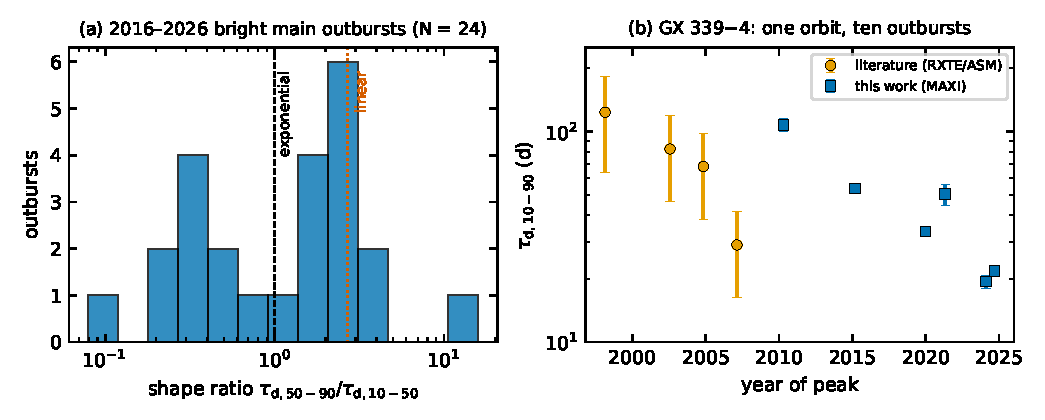
\includegraphics[width=\textwidth]{figures/fig4_shapes.pdf}
\caption{(a) Shape ratio $\tau_{\rm d,50-90}/\tau_{\rm d,10-50}$ of the 24 bright 2016--2026 main outbursts. The dashed line marks an exponential decay (1) and the dotted line a linear decay ($\simeq2.7$). (b) Decay times of the ten bright outbursts of GX~339$-$4 in the primary sample, from the literature (ASM; error bars include $\sigma_{\rm method}=0.19$\dex) and from this work (MAXI). One orbital period gives decay times that differ by a factor of six.}
\label{fig:shapes}
\end{figure*}

%=====================================================================
\section{Discussion}
\label{sec:discussion}

\subsection{What the null result means for the irradiated disc picture}
\label{sec:physics}

For the exponential phase, the irradiated disc model predicts $B\approx2/3$ if the outer disc is irradiation-dominated and $B\approx5/6$ for a viscously heated Kramers disc (Section~\ref{sec:theory}). Our data exclude both: $P(B\ge2/3)=0.006$, and $B=2/3$ lies above the 95 per cent upper limit in every leave-one-system-out fit and in both hierarchical models. The shallow limiting case, $B\simeq1/3$, lies inside our interval ($P(B\ge1/3)=0.16$), and our power to detect a slope of 0.3 was only 0.39. We therefore cannot exclude a weak dependence on disc size, and we do not claim that decay times are independent of it. What the data show is that the period is not the main factor. Across our period range of 1.42\dex, a slope of $1/3$ would change $\taud$ by 0.47\dex; the outbursts of GX~339$-$4 alone span 0.80\dex.

Several effects can produce such large variation, and can weaken the dependence on the orbit. In the model of \citet{KingRitter1998} the decay is exponential only while the X-rays ionize the disc to its edge. An outburst that starts with less mass in the disc, or reaches a lower peak, ionizes a smaller region, and its decay is then set by the peak luminosity rather than by the orbit \citep{Shahbaz1998}. The disc mass at the start of an outburst depends on how long the system has been in quiescence, and this differs between outbursts. Thermal winds driven by irradiation remove mass from the outer disc at a rate that changes during the outburst \citep{Tetarenko2018a,Dubus2019}. \citet{Tetarenko2018a} derived $\alpha$ from the decays of black hole outbursts with disc radii based on orbital periods, and found values that differ between systems. Differences in $\alpha$, or in the strength of irradiation \citep{Tetarenko2018b}, of a factor of a few would hide a slope of the size predicted. The $2/3$ and $5/6$ slopes assume that such quantities are similar from system to system, so our result can also be read as evidence that they are not.

Two limitations of the measurement point the same way. The 10--90 per cent decay time mixes an early phase, which may be exponential, with later phases that are often linear or slower, and the wide range of shape ratios (Section~\ref{sec:shapes}) shows that many decays are not single exponentials. The early-decay timescale $\tau_{\rm d,50-90}$ gives no clearer trend ($B=0.05$, $-0.54$ to $0.66$), but it is noisier. The measured quantity is also a band-limited flux, not the accretion rate: the BAT decay times are on median 0.61 of the MAXI ones, so the choice of band alone changes $\taud$ by about 0.2\dex. Many outbursts in the sample, including the influential GRS~1716$-$249, stayed in the hard state, where the irradiated-disc picture is less clearly applicable. A test that fits only the exponential part of soft-state decays, at similar peak Eddington ratios, may still reveal a dependence on disc size. It requires distances, masses and bolometric corrections, which we plan to add (Section~\ref{sec:limits}). Within GX~339$-$4, the decay times also appear to have become shorter over time (Fig.~\ref{fig:shapes}b), and testing them against peak flux and recurrence time is a natural next step.

\subsection{Comparison with earlier studies}
\label{sec:compare}

Our result agrees with \citet{YanYu2015}, who found no correlation between decay time and orbital period in the RXTE era, and extends it to the MAXI era with a formal test. It does not support the statement of \citet{Saraswati2025} that the decay time increases with orbital period. Three differences in analysis can explain this. First, we use a formal test with intrinsic scatter; a visual impression from a few points is easily driven by one or two long-period systems such as GRO~J1655$-$40. Second, \citet{Saraswati2025} included mini-outbursts, most of them below 0.1\,Crab, whose timescales are noisier. Third, one of their events belongs to a different source (Section~\ref{sec:confusion}). None of these choices creates a significant slope on its own in our data. Including all faint outbursts gives $B=-0.05$, and restricting the sample to dynamically confirmed black holes, as \citet{Saraswati2025} did, gives $B=0.00$. The peak fluxes listed by \citet{Saraswati2025} for outbursts after 2015 are 1.6--2.0 times ours for bright outbursts, and 4 times ours for GS~1354$-$64 in 2015. This suggests a difference in Crab normalization or band, which matters for which events pass a 0.1\,Crab limit.

\subsection{Reproducibility of two-point timescales}
\label{sec:repro}

The two-point e-folding time is simple and needs no model, which is why it is the standard for merging samples. Our validation shows that it is reproducible for simple, single-peaked outbursts but not for complex ones. Two groups that applied the same definition to the same ASM data agree to 0.10\dex\ (robust scatter) for most outbursts but differ by a factor of 4.6 for XTE~J1550$-$564 in 1998. The definition does not say which peak counts as the peak or where a re-flare ends, and these choices are rarely reported. We therefore recommend that future work (i) report the dates and fluxes of the selected 90, 50 and 10 per cent points, which our data release includes for every outburst, (ii) state how re-flares are separated, and (iii) include a method uncertainty, such as our $\sigma_{\rm method}$, when combining timescales from different groups. Without it, the published photon-noise errors, often below 0.01\dex, give literature values far too much weight in a combined fit. The cleanest solution is to remeasure the public ASM light curves with the same code as the MAXI data, which we leave to future work.

\subsection{Source confusion in MAXI light curves}
\label{sec:confusion}

The angular resolution of the MAXI GSC is about 1.5\degr\ \citep{Mihara2011}, so sources that are close on the sky can contaminate each other's light curves. \citet{Saraswati2025} list an outburst of GS~1354$-$64 that peaked at MJD 58524 with 1.92\,Crab. This date coincides with the peak of MAXI~J1348$-$630 (MJD 58523.5 in our data), a bright new transient 1.82\degr\ away. The BAT light curve of GS~1354$-$64 shows no outburst at that time: its median 15--50\,keV flux between MJD 58505 and 58545 was 0.005\,Crab. We conclude that this event belongs to MAXI~J1348$-$630, and we flag it, together with the corresponding MAXI windows of GS~1354$-$64. Similarly, the MAXI light curve of MAXI~J1631$-$479 has the same outburst history as 4U~1630$-$47, 0.6\degr\ away. We flag all its windows, and the 2019 outburst of 4U~1630$-$47, which overlapped with the outburst of MAXI~J1631$-$479. Catalogues built automatically from MAXI light curves should check every outburst of a source with a bright neighbour within about 2\degr, for example against BAT, which has a narrower point spread function.

\subsection{Limitations}
\label{sec:limits}

\begin{itemize}
\item \textit{Sample size.} Thirteen systems give limited power: a slope of 0.3 would be detected only about 40 per cent of the time. The upper limit on $B$ is the more robust result.
\item \textit{Selection against failed outbursts.} The 0.1\,Crab limit is applied in soft X-rays, where hard-state outbursts are faint. The 2013, 2017--18 and 2022 outbursts of GX~339$-$4 peaked at 0.03--0.06\,Crab in MAXI (2--10\,keV) but at 0.10--0.18\,Crab in BAT (15--50\,keV, three-day medians). Failed outbursts, about a third of all outbursts \citep{Alabarta2021}, are therefore under-represented in our sample and in both earlier samples. Including the faint events did not change the result.
\item \textit{Energy band and calibration.} Our 2--10\,keV band differs from the 2--12\,keV band of the literature, and the published MAXI-era peak fluxes differ from ours (Section~\ref{sec:compare}). The good agreement in $\taud$ with \citet{Saraswati2025} for most outbursts suggests that the effect on timescales is small, but a direct check with MAXI on-demand 2--12\,keV light curves remains to be done.
\item \textit{Orbital periods.} For five literature systems we used the periods tabulated by \citet{YanYu2015} or \citet{Saraswati2025} rather than reading them from the original papers. The two candidates have periods from X-ray dips, and GRS~1716$-$249 has a photometric period. Using only radial-velocity orbits gives $B=0.12$ ($-0.21$ to $0.50$).
\item \textit{Errors.} The Monte Carlo errors of two-point timescales are not always centred on the measured values (Section~\ref{sec:errors}), and the injection tests use single exponentials only.
\item \textit{Luminosity.} We have not converted peak fluxes to Eddington ratios, which needs distances, masses and a bolometric correction. Whether $\taud$ depends on the peak Eddington ratio, and whether that dependence differs between short and long periods, is left to future work.
\item \textit{Plan.} The analysis plan was fixed and fingerprinted before the test but not deposited in an external registry (Section~\ref{sec:stats}).
\end{itemize}

%=====================================================================
\section{Conclusions}
\label{sec:conclusions}

We measured uniform two-point rise and decay times for black hole and candidate outbursts observed by MAXI and Swift/BAT in 2016--2026. Combined with RXTE-era measurements, they allowed a formal test of whether decay times grow with orbital period, as the irradiated disc instability model predicts. Our main conclusions are as follows.
\begin{enumerate}
\item In 26 bright outbursts of 13 systems with $\porb=0.10$--$2.62$\,d, the decay time does not increase significantly with orbital period. The slope of $\log\taud$ against $\log\porb$ is $0.17$ ($-0.17$ to $0.52$, 95 per cent), and a constant decay time of about 30\,d describes the data as well as a power law. This holds in every robustness check.
\item Slopes of $2/3$ and $5/6$, expected for the exponential phase of irradiated and viscously heated discs, are excluded (posterior probabilities 0.006 and 0.001), and $B=2/3$ is excluded at 95 per cent in every leave-one-system-out fit. A shallow slope near $1/3$ remains allowed.
\item The scatter in decay time between outbursts of the same system (0.27\dex, pooled over four systems and dominated by GX~339$-$4) is as large as the scatter between systems, and no additional scatter between systems is needed. The decay time of an outburst is therefore set mainly by the conditions of that outburst, with the orbit at most a minor factor. Rise times, in contrast, differ more between systems than between outbursts.
\item The two-point e-folding time is reproducible to about 0.05--0.10\dex\ for single-peaked outbursts, but two groups using the same definition and data differ by up to a factor of 4.6 for complex outbursts. Combined analyses should include a method uncertainty and report the selected points.
\item A published 2019 outburst of GS~1354$-$64 belongs to MAXI~J1348$-$630, and the MAXI light curve of MAXI~J1631$-$479 is dominated by 4U~1630$-$47. Catalogues built from MAXI light curves need confusion checks.
\end{enumerate}
The catalogue, the code and the analysis plan are public, so that the test can be repeated as new periods are measured and new outbursts occur.

%=====================================================================
\section*{Acknowledgements}

This research used MAXI data provided by RIKEN, JAXA and the MAXI team, and Swift/BAT transient monitor results provided by the Swift/BAT team. It made use of the BlackCAT catalogue and of NASA's Astrophysics Data System. The analysis used \textsc{numpy} \citep{Harris2020}, \textsc{scipy} \citep{Virtanen2020}, \textsc{pandas} \citep{McKinney2010}, \textsc{astropy} \citep{Astropy2022}, \textsc{emcee} \citep{ForemanMackey2013} and \textsc{matplotlib} \citep{Hunter2007}.

\textit{Use of AI tools.} An AI assistant (Claude, Anthropic) was used to write the analysis code, to search for and check references, to review the analysis, and to draft the text of this manuscript. The author checked the code, the results and the citations and takes full responsibility for the content.

\textit{Author contributions.} B.~[Surname]: conceptualization, data curation, formal analysis, investigation, methodology, software, validation, visualization, writing (original draft, review and editing).

\textit{Funding.} This work received no specific funding.

\textit{Conflict of interest.} The author declares no conflict of interest.

\textit{Ethics.} This work uses only public astronomical data and involves no human or animal subjects.

\section*{Data Availability}

The MAXI and Swift/BAT light curves are public at \url{http://maxi.riken.jp} and \url{https://swift.gsfc.nasa.gov/results/transients/}. The full measurement table (all outburst windows, with the dates and fluxes of the selected 90, 50 and 10 per cent points, all rise and decay timescales with Monte Carlo ranges, shape ratios and BAT decay times), the system-parameter table with a reference for every value, the transcribed literature timescales, the analysis plan with its SHA-256 fingerprint, and all code needed to reproduce the figures and tables will be made available at [repository URL, to be added on submission].

\bibliographystyle{mnras}
\bibliography{references}

\bsp
\label{lastpage}
\end{document}
